% TeX encoding = utf8
% TeX spellcheck = pl_PL 
\documentclass[a4paper,titlepage,11pt,twosides,floatssmall]{mwrep}
\usepackage[left=2.5cm,right=2.5cm,top=2.5cm,bottom=2.5cm]{geometry}
\usepackage[OT1]{fontenc}
\usepackage{polski}
\usepackage{amsmath}
\usepackage{amsfonts}
\usepackage{amssymb}
\usepackage{graphicx}
\usepackage{url}
\usepackage{tikz}
\usetikzlibrary{arrows,calc,decorations.markings,math,arrows.meta}
\usepackage{rotating}
\usepackage[percent]{overpic}
\usepackage[utf8]{inputenc}
\usepackage{xcolor}
\usepackage{pgfplots}
\usetikzlibrary{pgfplots.groupplots}
\usepackage{listings}
\usepackage{matlab-prettifier}
\usepackage{siunitx}
\usepackage[section]{placeins}
\definecolor{szary}{rgb}{0.95,0.95,0.95}
\SendSettingsToPgf
\sisetup{detect-weight,exponent-product=\cdot,output-decimal-marker={,},per-mode=symbol,binary-units=true,range-phrase={-},range-units=single}

%konfiguracje pakietu listings
\lstset{
	backgroundcolor=\color{szary},
	frame=single,
	breaklines=true,
}
\lstdefinestyle{customlatex}{
	basicstyle=\footnotesize\ttfamily,
	%basicstyle=\small\ttfamily,
}
\lstdefinestyle{customc}{
	breaklines=true,
	frame=tb,
	language=C,
	xleftmargin=0pt,
	showstringspaces=false,
	basicstyle=\small\ttfamily,
	keywordstyle=\bfseries\color{green!40!black},
	commentstyle=\itshape\color{purple!40!black},
	identifierstyle=\color{blue},
	stringstyle=\color{orange},
}
\lstdefinestyle{custommatlab}{
	captionpos=t,
	breaklines=true,
	frame=tb,
	xleftmargin=0pt,
	language=matlab,
	showstringspaces=false,
	%basicstyle=\footnotesize\ttfamily,
	basicstyle=\scriptsize\ttfamily,
	keywordstyle=\bfseries\color{green!40!black},
	commentstyle=\itshape\color{purple!40!black},
	identifierstyle=\color{blue},
	stringstyle=\color{orange},
}

%wymiar tekstu (bez żywej paginy)
\textwidth 160mm \textheight 247mm

%ustawienia pakietu pgfplots
\pgfplotsset{
	tick label style={font=\scriptsize},
	label style={font=\small},
	legend style={font=\small},
	title style={font=\small}
}

\def\figurename{Rys.}
\def\tablename{Tab.}

%konfiguracja liczby pływających elementów
\setcounter{topnumber}{0}%2
\setcounter{bottomnumber}{3}%1
\setcounter{totalnumber}{5}%3
\renewcommand{\textfraction}{0.01}%0.2
\renewcommand{\topfraction}{0.95}%0.7
\renewcommand{\bottomfraction}{0.95}%0.3
\renewcommand{\floatpagefraction}{0.35}%0.5

\begin{document}
	
	\begin{titlepage}
		\begin{center}
			\Huge{\textsc{Sprawozdanie z pierwszej części projektu z przedmiotu \\,,Technika Automatyzacji Procesów''}} \\
			[15cm]
			\Large{Numer zadania: 3 \\Wykonawcy:}\\
			\Large{Dawidiuk Marek \\ Giełdowski Daniel \\ Kłos Maciej \\ Taras Sylwia}
		\end{center}
	\end{titlepage}
	
	\tableofcontents
	\newpage
	\chapter{Opis otrzymanego modelu}

W ramach tego projektu analizowaliśmy otrzymany model obiektu znanego jako reaktor przepływowy. Obiekt składa się z pojemnika wypełnionego cieczą z rozpuszczoną nieokreśloną substancją. Do pojemnika wpływa strumieniem $F_{in}$ ciecz o określonej temperaturze $T_{in}$ oraz stężeniu rozpuszczonej substancji $C_{Ain}$. W pojemniku jest określona ilość cieczy $V$ w określonej temperaturze $T$. Ciecz z pojemnika wypływa strumieniem $F$, zawierając stężenie $C_A$ rozpuszczonej substancji. Dodatkowo przez pojemnik przeprowadzona jest rura odpowiedzialna za chłodzenie bądź podgrzewanie, którą strumieniem $F_C$ płynie ciecz o temperaturze wejściowej $T_{Cin}$.\\\\ Obiekt opisany jest następującymi równaniami:

\begin{equation}
	\left\{
	\begin{tabular}{l}
	$V \cdot \frac{dC_A}{dt}=F_{in} \cdot C_{Ain}-F \cdot C_A-V \cdot k_0 \cdot e^{-\frac{E}{R \cdot T}} \cdot C_A$\\
	$V \cdot \rho \cdot c_p \cdot \frac{dT}{dt}=F_{in} \cdot \rho \cdot c_p \cdot T_{in}-F \cdot \rho \cdot c_p \cdot T+V \cdot h \cdot k_0 \cdot e^{-\frac{E}{R \cdot T}} \cdot C_A - \frac{a \cdot (F_C)^{b+1}}{F_C+\frac{a \cdot (F_C)^b}{2 \cdot \rho_c \cdot c_{pc}}} \cdot (T-T_{Cin})$
	\end{tabular}
	\right.
\end{equation}
W równaniach występują stałe o podanych wartościach:\\
\begin{itemize}
	\item $\rho=\rho_c=10^6\frac{g}{m^3}$
	\item $c_p=c_{pc} = 1 \frac{cal}{g\cdot K}$
	\item $k_0 = 10^{10} \frac{1}{min}$
	\item $\frac{E}{R} = 8330,1 \frac{1}{K}$
	\item $h = 130\cdot 10^6 \frac{cal}{kmol}$
	\item $a = 1,678\cdot 10^6\frac{cal}{K\cdot m^3}$
	\item $b = 0,5$
\end{itemize}
Na potrzeby linearyzacji otrzymaliśmy także dane odnośnie wartości zmiennych modelu w zadanym punkcie pracy układu:\\
\begin{itemize}
	\item $V=1m^3$
	\item $F_{in} = F = 1 \frac{m^3}{min}$
	\item $C_{Ain} = 2 \frac{kmol}{m^3}$
	\item $F_C = 15 \frac{m^3}{min}$
	\item $T_{in} = 323K$
	\item $T_{Cin} = 365K$
	\item $C_A = 0,26\frac{kmol}{m^3}$
	\item $T = 393,9K$
\end{itemize}
W ramach zadania wielkości te podzielone zostały na 4 grupy:\\
\begin{itemize}
	\item stałe - $V,F,F_{in}$
	\item regulowane - $C_A,T$
	\item sterujące - $C_{Ain},F_C$
	\item zakłócenia - $T_{in},T_{Cin}$
\end{itemize}
Po zastąpieniu stałych w równaniach liczbami, otrzymywany jest następujący układ równań:\\
\begin{equation}
	\left\{
	\begin{tabular}{l}
	$\frac{dC_A}{dt} = C_{Ain} - C_A - 10^{10}\cdot e^{-\frac{8330,1}{T}}\cdot C_A$\\
	$\frac{dT}{dt} = T_{in} - T + 130\cdot 10^{10}\cdot e^{-\frac{8330,1}{T}}\cdot C_A-\frac{1,678\cdot (F_C)^{1,5}}{F_C+0,839\cdot (F_C)^{0,5}}(T-T_{Cin})$
	\end{tabular}
	\right.
\end{equation}
Ostatnią rzeczą jaka musiała zostać wzięta pod uwagę było dokładniejsze określenie wartości wyjść w punkcie pracy, ponieważ te podane w zadaniu były przybliżone. Ustawiając wszystkie zmienne (prócz wyjściowych) na podane wartości, po ustabilizowaniu wyjścia wyniosły w przybliżeniu $C_A = 0,2646$ oraz $T = 393,9531$.

	\chapter{Model liniowy}
\section{Równania stanu}
W celu opracowania modelu liniowego obiektu wykonaliśmy linearyzację w zadanym punkcie pracy. Pamiętając, że pochodna w tym punkcie wynosi 0, otrzymaliśmy następujące równania.

\begin{equation}
\left\{
\begin{tabular}{l}
$\frac{dC_A}{dt} = (-1-10^{10}\cdot e^{-\frac{8330.1}{T_0}})(C_A-C_{A0})+(-10^{10}\cdot e^{-\frac{8330.1}{T_0}}\cdot \frac{8330.1}{T_0^2}\cdot C_{A0})(T-T_0)+(C_{Ain}-C_{Ain0})$\\\\
$\frac{dT}{dt} = (130\cdot 10^{10}\cdot e^{-\frac{8330.1}{T_0}})(C_A-C_{A0}) + (-1+130\cdot 10^{10}\cdot e^{-\frac{8330.1}{T_0}}\cdot \frac{8330.1}{T_0^2}\cdot C_{A0}-\frac{1.678\cdot (F_C)^{1.5}}{F_C+0.839\cdot (F_C)^{0.5}})(T-T_0)$\\\\
$\quad + (-1.678(T_0-T_{Cin0})(\frac{1.5\cdot (F_{C0})^{0.5}}{F_{C0}+0.839\cdot (F_{C0})^{0.5}}-\frac{ (F_{C0})^{1.5}}{(F_{C0}+0.839\cdot (F_{C0})^{0.5})^2}\cdot (1+0.5\cdot 0.839 \cdot (F_{C0})^{-0.5})))(F_C-F_{C0})$\\\\
$\quad + (T_{in} - T_{in0}) + (\frac{1.678\cdot (F_C)^{1.5}}{F_C+0.839\cdot (F_C)^{0.5}})(T_{Cin} - T_{Cin0})$\\\\
\end{tabular}
\right.
\end{equation}
Podstawiając wartości w punkcie pracy (zmienne z indeksem 0) otrzymujemy:
\begin{equation}
\left\{
\begin{tabular}{l}
$\frac{dC_A}{dt} = -7.5597(C_A-0.2646)-0.0932(T-393.9531)+(C_{Ain}-2)$\\\\
$\frac{dT}{dt} = 852.7638(C_A-0.2646) + 5.7693(T-393.9531) -6.0732(F_C-15) + (T_{in} - 323) + 5.3417(T_{Cin} - 365)$\\\\
\end{tabular}
\right.
\end{equation}

\begin{equation}
\left\{
\begin{tabular}{l}
$\frac{dC_A}{dt} = -7.5597\cdot C_A-0.0932\cdot T+C_{Ain} + 36.7167$\\\\
$\frac{dT}{dt} = 852.7638\cdot C_A + 5.7693\cdot T -6.0732\cdot F_C + T_{in} + 5.3417\cdot T_{Cin} - 4680.0974$\\\\
\end{tabular}
\right.
\end{equation}
\newpage
\section{Transmitancja}
Mając model w postaci układu równań wykorzystaliśmy możliwości Matlaba do obliczania transmitancji (funkcja $ss()$). W tym celu określiliśmy macierze:
\begin{equation}
	A=\left[
	\begin{tabular}{c c}
	-7.5597&-0.0932\\852.7638&5.7693
	\end{tabular}
	\right]
\end{equation}
\begin{equation}
B=\left[
\begin{tabular}{c c c c}
1&0&0&0\\0&-6.0732&1&5.3417
\end{tabular}
\right]
\end{equation}
\begin{equation}
C=\left[
\begin{tabular}{c c}
1&0\\0&1
\end{tabular}
\right]
\end{equation}
\begin{equation}
D=\left[
\begin{tabular}{c c c c}
0&0&0&0\\0&0&0&0
\end{tabular}
\right]
\end{equation}
Wyliczone transmitancje to:
\begin{equation}
	\frac{C_A(s)}{C_{Ain}(s)} = \frac{s-5.769}{s^2+1.79s+35.83}
\end{equation}
\begin{equation}
\frac{C_A(s)}{F_C(s)} = \frac{0.5658}{s^2+1.79s+35.83}
\end{equation}
\begin{equation}
\frac{C_A(s)}{T_{in}(s)} = \frac{-0.09316}{s^2+1.79s+35.83}
\end{equation}
\begin{equation}
\frac{C_A(s)}{T_{Cin}(s)} = \frac{-0.4976}{s^2+1.79s+35.83}
\end{equation}
\begin{equation}
\frac{T(s)}{C_{Ain}(s)} = \frac{8.52.8}{s^2+1.79s+35.83}
\end{equation}
\begin{equation}
\frac{T(s)}{F_C(s)} = \frac{-6.073s-45.91}{s^2+1.79s+35.83}
\end{equation}
\begin{equation}
\frac{T(s)}{T_{in}(s)} = \frac{s + 7.56}{s^2+1.79s+35.83}
\end{equation}
\begin{equation}
\frac{T(s)}{T_{Cin}(s)} = \frac{5.342 s + 40.38}{s^2+1.79s+35.83}
\end{equation}
\newpage
\section{Porównanie modelu nieliniowego i liniowego}
Po zaimplementowaniu modelu w postaci równań stanu w Matlabie, wykonaliśmy eksperymenty polegające na zmianie wartości jednej ze zmiennych sterujących. Na wykresach od \ref{fig:lincacain0} do \ref{fig:lintfc0} przedstawione zostały przebiegi wyjść dla małych zmian zmiennych sterujących. Jak widać model ten radzi sobie w tym zakresie zadowalająco. Odchyły stężenia $C_A$ względem modelu nieliniowego nie są duże, i mieszczą się w zakresie $<-0.01;0.01>$. Różnica temperatury $T$ między modelami nie przekracza jednego stopnia Kelwina. Przebiegi dla obydwu modeli są także podobne kształtem.

Inaczej przedstawia się sytuacja dla dużych skoków sterowania, przedstawiona na wykresach od \ref{fig:lincacain1} do \ref{fig:lintfc1}. Odchylenie modelu liniowego od nieliniowego jest ewidentnie większe, i  w większości przypadków kształt przebiegów nie pokrywa się pomiędzy modelami. Na szczególną uwagę zasługuje tu wykres \ref{fig:lintcain1}, ponieważ tylko na nim wartość końcowa wyjścia $T$ modelu liniowego jest zbliżona do wartości dla modelu nieliniowego. Oznacza to, że w teorii model liniowy powinien dosyć dobrze odwzorowywać wartość wyjścia $T$ przy skokach sterowania $C_{Ain}$.

\begin{figure}
	\centering
	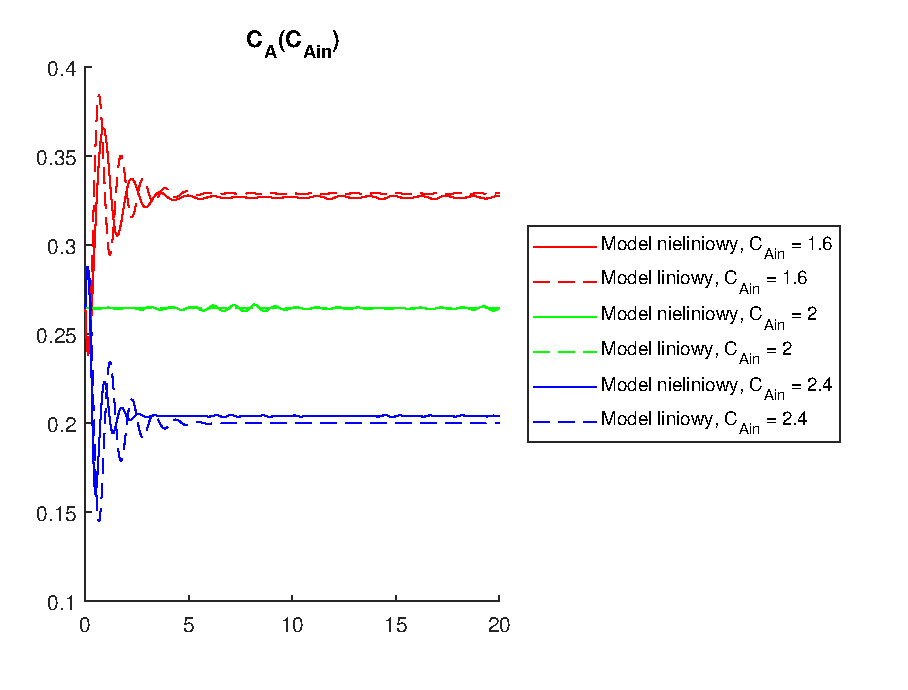
\includegraphics[width=.8\linewidth]{plot/lin_cacain_0.eps}
	\caption{Porównanie wyjścia $C_A$ modelu nieliniowego i liniowego dla skoku sterowania $C_{Ain}$ blisko punktu pracy}
	\label{fig:lincacain0}
\end{figure}
\begin{figure}
\centering
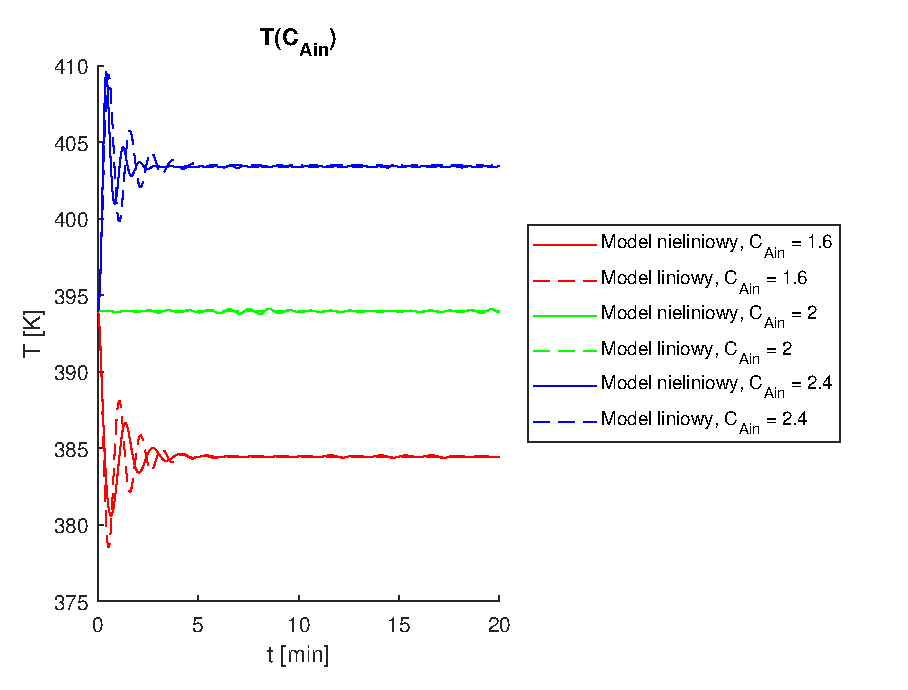
\includegraphics[width=.8\linewidth]{plot/lin_tcain_0.eps}
\caption{Porównanie wyjścia $T$ modelu nieliniowego i liniowego dla skoku sterowania $C_{Ain}$ blisko punktu pracy}
\label{fig:lintcain0}
\end{figure}
\begin{figure}
\centering
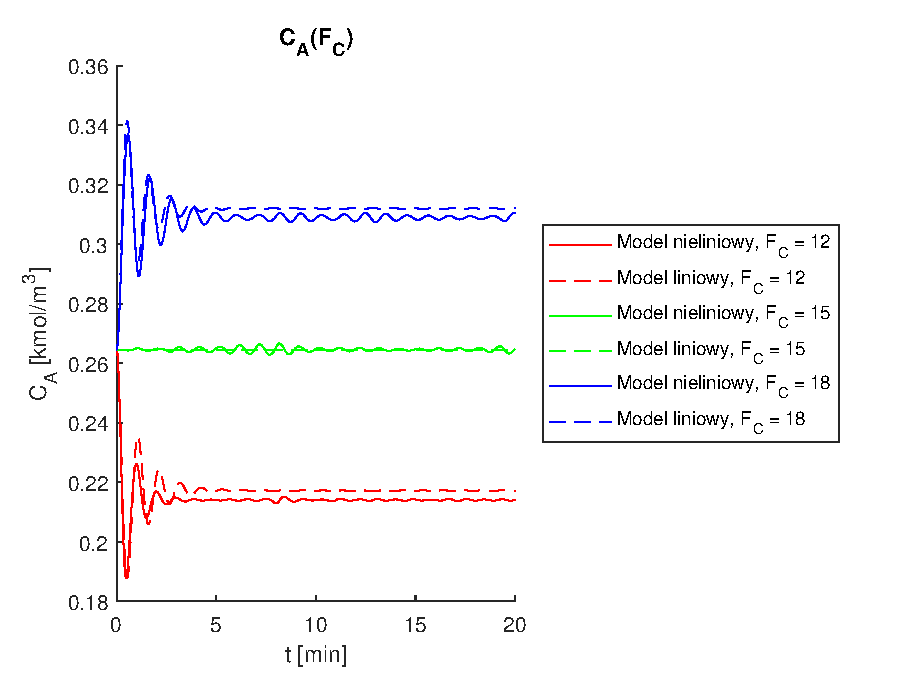
\includegraphics[width=.8\linewidth]{plot/lin_cafc_0.eps}
\caption{Porównanie wyjścia $C_A$ modelu nieliniowego i liniowego dla skoku sterowania $F_C$ blisko punktu pracy}
\label{fig:lincafc0}
\end{figure}
\begin{figure}
\centering
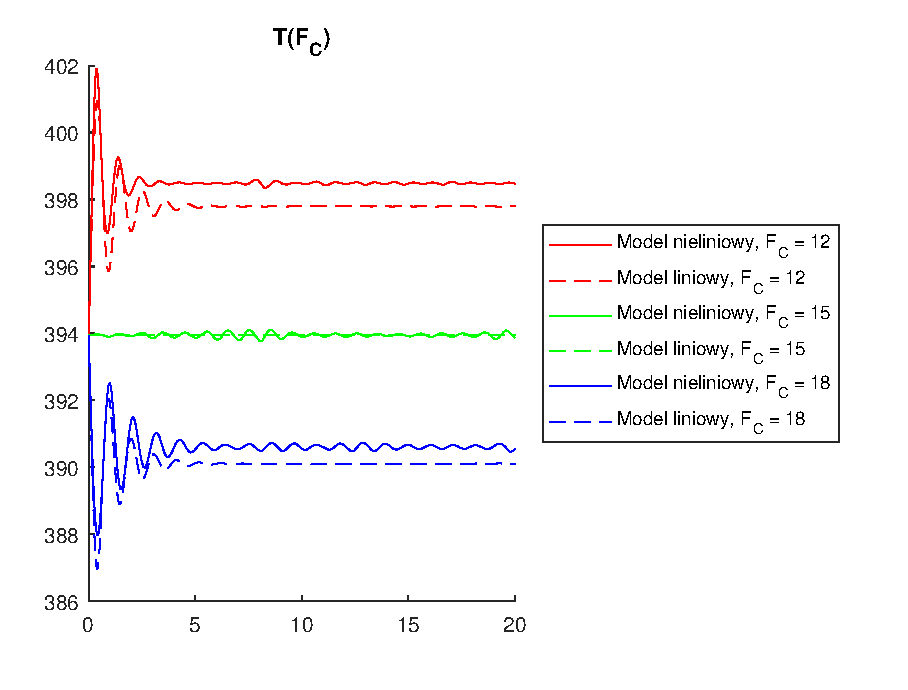
\includegraphics[width=.8\linewidth]{plot/lin_tfc_0.eps}
\caption{Porównanie wyjścia $T$ modelu nieliniowego i liniowego dla skoku sterowania $F_C$ blisko punktu pracy}
\label{fig:lintfc0}
\end{figure}

\begin{figure}
	\centering
	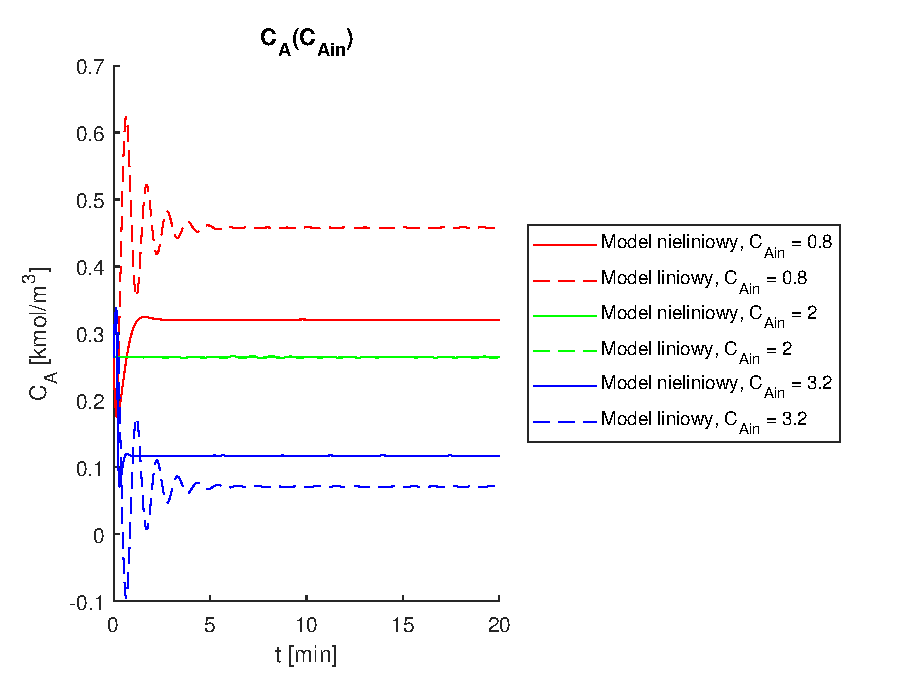
\includegraphics[width=.8\linewidth]{plot/lin_cacain_1.eps}
	\caption{Porównanie wyjścia $C_A$ modelu nieliniowego i liniowego dla skoku sterowania $C_{Ain}$ daleko od punktu pracy}
	\label{fig:lincacain1}
\end{figure}
\begin{figure}
	\centering
	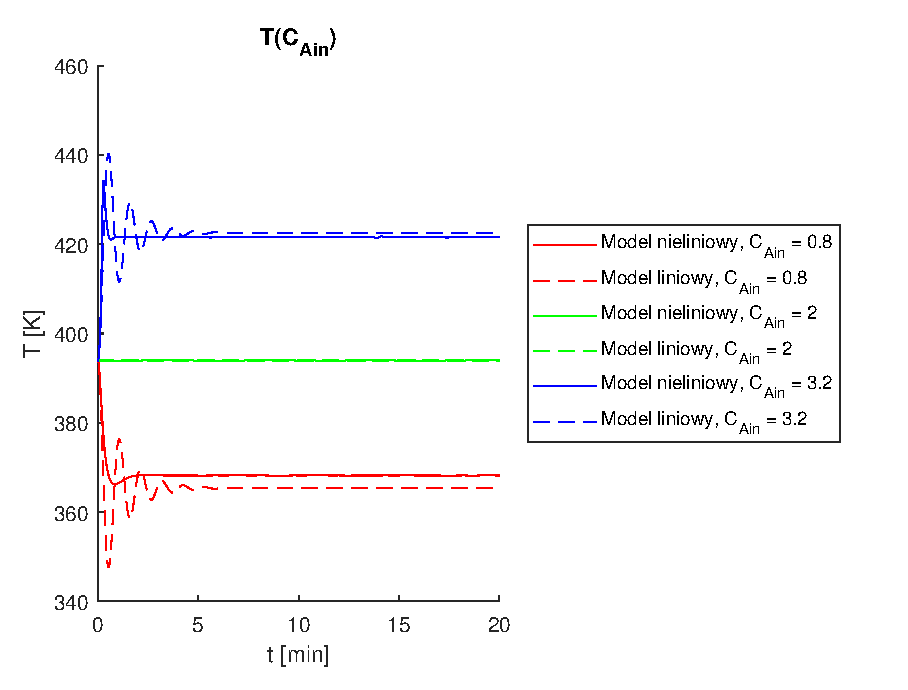
\includegraphics[width=.8\linewidth]{plot/lin_tcain_1.eps}
	\caption{Porównanie wyjścia $T$ modelu nieliniowego i liniowego dla skoku sterowania $C_{Ain}$ daleko od punktu pracy}
	\label{fig:lintcain1}
\end{figure}
\begin{figure}
	\centering
	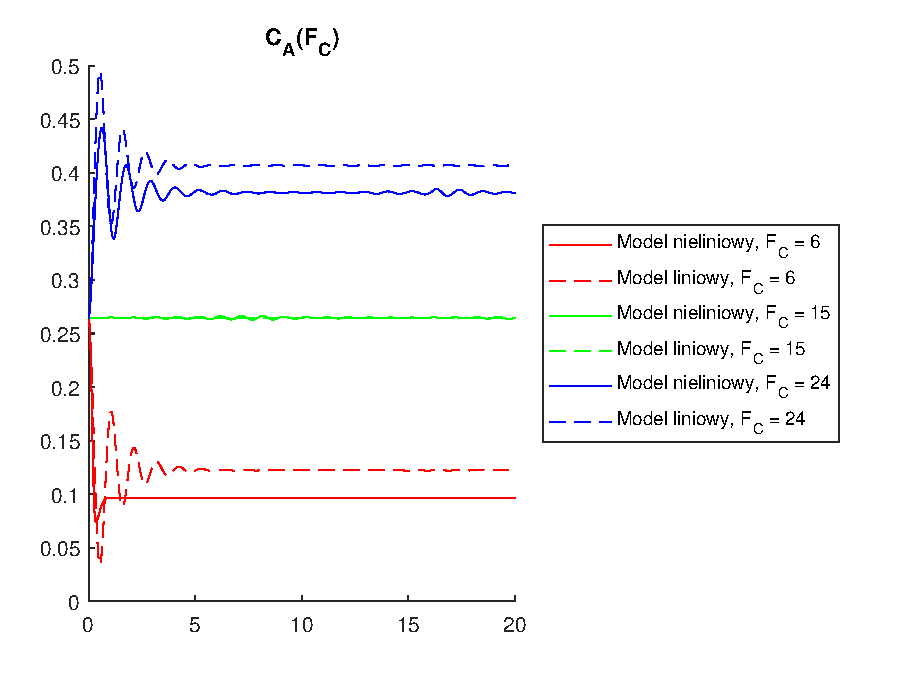
\includegraphics[width=.8\linewidth]{plot/lin_cafc_1.eps}
	\caption{Porównanie wyjścia $C_A$ modelu nieliniowego i liniowego dla skoku sterowania $F_C$ daleko od punktu pracy}
	\label{fig:lincafc1}
\end{figure}
\begin{figure}
	\centering
	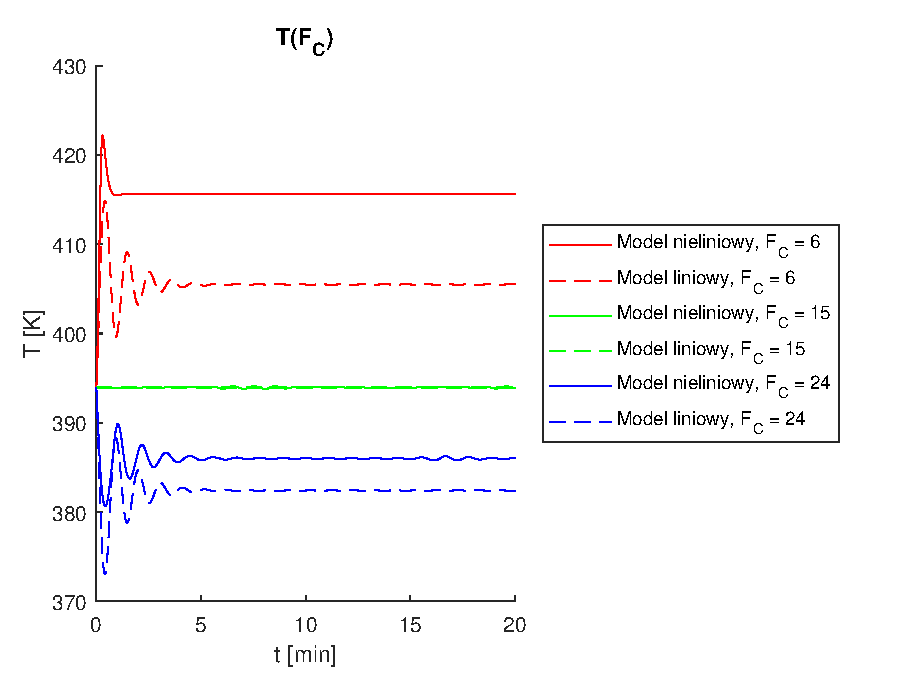
\includegraphics[width=.8\linewidth]{plot/lin_tfc_1.eps}
	\caption{Porównanie wyjścia $T$ modelu nieliniowego i liniowego dla skoku sterowania $F_C$ daleko od punktu pracy}
	\label{fig:lintfc1}
\end{figure}
	
\end{document}